\section{Sim-to-real Transfer}
The training of state-based RL policies typically relies on privileged information which is not accessible in real-world deployment scenarios. Consequently, it is imperative to distill the state-based policy into a visual policy for achieving sim2real transfer. 


\begin{figure*}[t]
  \centering
  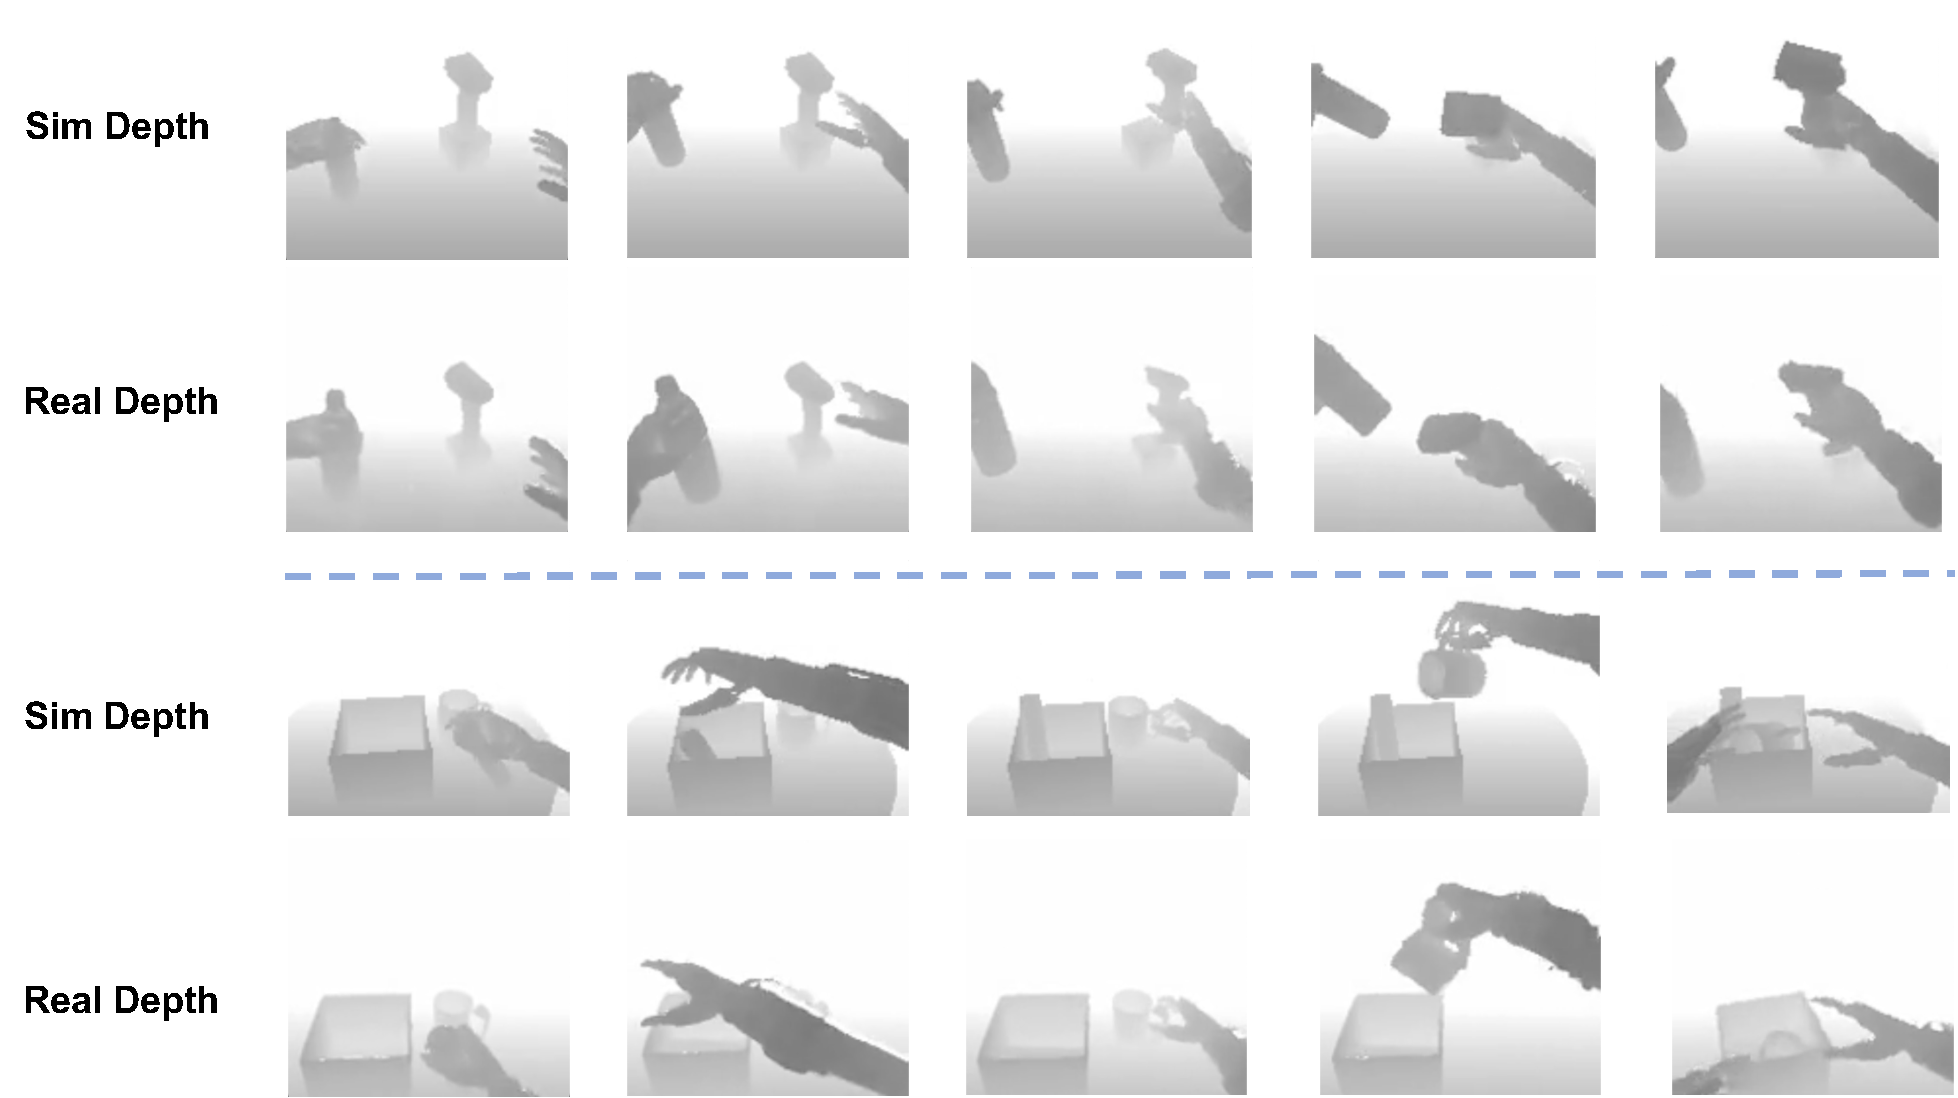
\includegraphics[width=1.0\linewidth]{figures/compare_depth_pic.pdf}
  \vspace{-15pt}
  \caption{\textbf{Depth image visualization.} We present a visual comparison between simulated and real-world depth maps across two different tasks. Notably, after applying our preprocessing pipeline, the depth representations of the hand and object exhibit a strong semantic correspondence, highlighting the efficacy of \ourshort in bridging the sim2real gap.}
  \label{fig:compare_depth}
\end{figure*}


\begin{figure}[h]
  \centering
  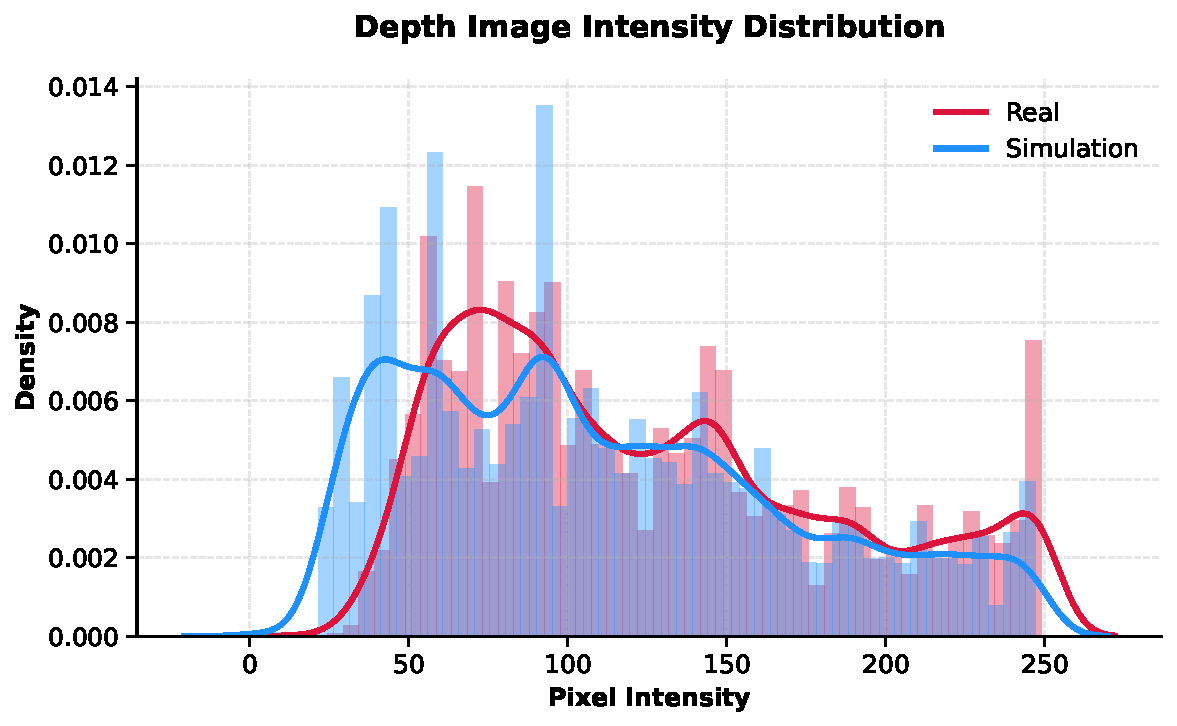
\includegraphics[width=1.0\linewidth]{figures/depth_dist_pic.pdf}
  \vspace{-15pt}
  \caption{\textbf{Depth intensity distribution. }The horizontal axis represents the depth values, while the vertical axis indicates their corresponding proportions. This figure illustrates that the depth distributions derived from simulation and real-world images exhibit a notable resemblance in value patterns.}
  \label{fig:depth_dist}
\end{figure}
\subsection{Leveraging Depth Image as Visual Input}
Prior work~\cite{lumdextrah,zhuang2023robot,zhuanghumanoid,rudin2025parkour} has explored the use of depth images
for vision-based sim2real transfer. However, they often necessitate intricate and highly customized augmentation strategies to bridge the gap. In this work, we introduce a more versatile, manipulation-tailored egocentric depth-image augmentation method. Specifically, we clip depth values beyond a threshold distance $\mathbf{d}$~(set per task). For real depth images, missing depth values resulting from edge capture failures are filled in with the maximum depth. To emulate real-world edge noise and blur in simulation, we augment simulated depth images by adding Gaussian noise and Gaussian blur during training. Additionally, to mimic missing depth values, we randomly set 0.5\% of pixel values in simulation-rendered images to the maximum depth. To enrich the diversity of depth-noise distributions, we further employ the NYU Depth Dataset~\cite{silberman2012indoor} and adopt a mixup strategy that linearly blends the simulation-rendered depth image $\boldsymbol{o}_{sim}$ with a certain data depth map $\boldsymbol{o}_{dataset}$: ${\boldsymbol{\hat{o}}} = \alpha*\boldsymbol{o}_{sim} + (1 - \alpha)*\boldsymbol{o}_{dataset}$, where $\alpha$ is the coefficient. As illustrated in Figure~\ref{fig:compare_depth}, our augmentation  not only semantically aligns simulated renderings with real-world depth images, but also preserves crucial depth disparity cues essential for accurate visuomotor control. 

Furthermore, we visualize the distribution of depth values under similar frames in both simulation and real-world settings. As illustrated in Figure~\ref{fig:depth_dist}, our processing approach leads to a close alignment in value distributions between real-world and simulated depth images, indicating a reduced sim2real gap. 





\subsection{DAgger Distillation Training}

In DAgger training, the state-based expert policy acts as the teacher to guide the learning of a visual student policy.  In contrast to prior approaches that distill to object masks or segmented images, \ourshort directly distills the state into raw visual observations of entire visual scenarios. This design obviates the need for explicit camera calibration and facilitates the acquisition of the robot's in-the-wild generalization capabilities. Furthermore, we introduce a series of auxiliary design choices aimed at enhancing both the asymptotic performance of DAgger training. 

\textbf{Model architecture: } The input observations are rendered at a resolution of $140\times 140$ pixels and subsequently stacked into sequences of 3 consecutive frames before being passed to the image encoder. Consistent with the design of Yuan et al.~\cite{yuanlearning,yuan2022pre}, we utilize the first two layers of a ResNet‑18 encoder~\cite{he2016deep} to more effectively capture fine‑grained visual details. Moreover, to ensure distributional consistency between training and evaluation phases, we replace all BatchNorm layers in the encoder with GroupNorm~\cite{wu2018group}.

\textbf{Trajectory rollout scheduler:} At the beginning of DAgger training, we adopt the expert policy to roll out trajectories for supervising the student. As training progresses, the reliance on expert rollouts is gradually reduced by annealing the probability $p$, while proportionally increasing the student policy's participation in rollouts. The pseudocode for the DAgger training procedure is presented in Algorithm~\ref{alg:training}, where $N_{\text{epochs}}$ denotes the total number of training epochs, $T$ represents the trajectory rollout intervals, and $\mathcal{D}$ refers to the replay buffer. At each interaction step with the environment,
the action $a$ is determined by the trajectory rollout scheduler, which probabilistically selects between the student actions $a_{\text{student}}$ and expert actions $a_{\text{expert}}$ based on a dynamically adjusted probability $p$. Here, we employ an exponential decay schedule to reduce the probability. 

\begin{algorithm}
\caption{DAgger Distillation Training}\label{alg:training}
\begin{algorithmic}

\State $\mathcal{D} \gets \emptyset$
\State $\text{trajectory rollout scheduler } \mathcal{S} \gets \text{Scheduler}(p_0)$
\For{$n \gets 0$ to $N_{\text{epochs}}$} 
    \For{$t \gets 0$ to  $T$} \Comment{Rollout Trajectory}
        \State $a_{\text{student}} \gets \pi_\text{student}(o_{\text{student}})$
        \State $a_{\text{expert}} \gets \pi_\text{expert}(o_{\text{expert}})$
        \State $a \gets \mathcal{S}$.\textproc{random\_choose} $(a_{\text{student}}, a_{\text{expert}}, p_t)$
        
        \State $\mathcal{D} \gets \mathcal{D} \cup \{(o_{\text{student}}, a_{\text{expert}})\}$
        \State $o_{\text{student}, t+1}, o_{\text{expert}, t+1} \gets$ \textproc{env.step}($a$)
        \State $p_{t+1} \gets \mathcal{S}$.\textproc{step}$()$ 
    %     \State $t \gets t+1$
    \EndFor
    \State $\pi_\text{student} \gets \textproc{update}(\pi_\text{student}, \mathcal{D})$ \Comment{Policy Training}
\EndFor
\end{algorithmic}
\end{algorithm}

We jointly optimize the student policy using a combination of L1 and L2 action loss terms. Additionally, to mitigate the  overfitting to the low-dimensional states, we inject uniform noise into the proprioception states during training. More details and experimental results can be found in Appendix~\ref{sec:dagger} and Appendix~\ref{sec:dagger_train}. 

\begin{figure}[h]
  \centering
  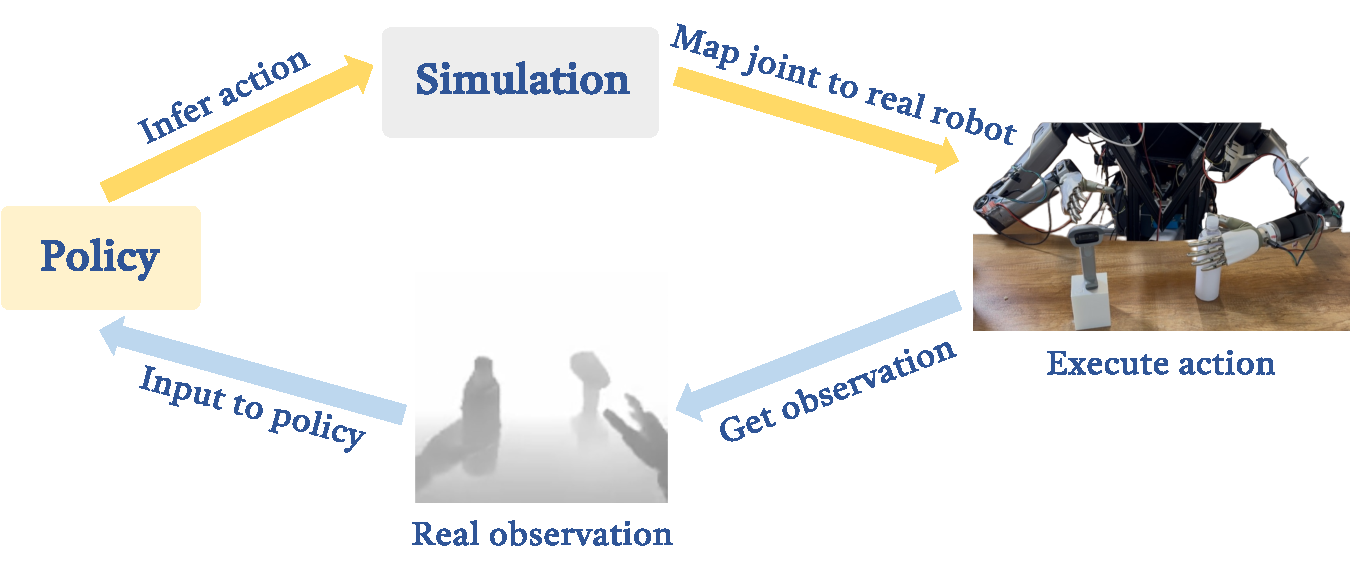
\includegraphics[width=1.0\linewidth]{figures/control_pic.pdf}
  \vspace{-15pt}
  \caption{\textbf{Hybrid Sim2real Control.} We leverage real-world observations to infer actions and utilize simulation to compute the corresponding joint values, which are subsequently mapped onto the real robots. This hybrid strategy effectively mitigates the sim2real gap.}
  \label{fig:control}
\end{figure}
\subsection{Hybrid Sim2real Control}
Given the quasi-static nature of our tasks, we adopt a hybrid control strategy to mitigate the gap between simulation and real-world dynamics: real-world visual observations are used to infer the actual action, which is then applied to the simulation environment to perform a forward step. The updated joint positions of the simulated robot are subsequently transferred to the real robot for execution. Following this, the camera captures the image of the updated physical status of the real robot and incorporates the proprioception states as the input observation for the next inference cycle. The pseudocode of our control is provided in Algorithm~\ref{alg:control}.
By sharing the same Inverse Kinematics~(IK) method and dynamic parameters across simulation and the real world, this approach not only enables the policy to adapt its behavior based on real-world environmental variations but also effectively narrows the sim2real discrepancy. The pipeline is shown in Figure~\ref{fig:control}. 


 


\begin{algorithm}
\caption{Hybrid Sim2real Control}\label{alg:control}
\begin{algorithmic}


\For{$t \gets 0$ to  $T$} \Comment{Real-world Policy Execution}
    \State $a_{t} \gets \pi_\text{policy}(o_{\text{real\_obs},t})$
     \State $o_{\text{sim}, t+1} \gets$ \textproc{env.step}($a_{t}$)
    \State $\mathcal{J}_{\text{all\_joints}} \gets$  \textproc{get\_all\_current\_joint\_qpos\_in\_sim}()
    \State $o_{\text{real\_obs},t+1} \gets$ \textproc{set\_all\_qpos\_in\_real}($\mathcal{J}_{\text{all\_joints}}$)
\EndFor
\end{algorithmic}
\end{algorithm}